% 
\documentclass[aspectratio=169]{beamer}
\usetheme{WG}
\usepackage[english,russian]{babel}
\usepackage[utf8]{inputenc}
\usepackage{verbatim}
\usepackage{graphicx}
\usepackage{pgfpages}
\usepackage{ulem}
\usepackage{float}
\usepackage{amsmath}

% quote author
\usepackage{amsthm} % pushQED, popQED
\newenvironment{aquote}[1]{%
  \pushQED{#1}%
  \begin{quote}
}{%
  \noindent\hfill(\popQED)%
  \end{quote}%
}

\definecolor{mygreen}{RGB}{0,150,0}
\definecolor{myyellow}{RGB}{120,120,0}

\usepackage{listings}
\definecolor{light-gray}{gray}{0.95}
\lstset{
language=Python,                             % Code langugage
basicstyle=\small\ttfamily,                   % Code font, Examples: \footnotesize, \ttfamily
keywordstyle=\color{WGred},        % Keywords font ('*' = uppercase)
commentstyle=\color{gray},              % Comments font
numbers=left,                           % Line nums position
numberstyle=\tiny,                      % Line-numbers fonts
stepnumber=1,                           % Step between two line-numbers
numbersep=5pt,                          % How far are line-numbers from code
backgroundcolor=\color{light-gray}, % Choose background color
frame=lines,                             % A frame around the code
tabsize=4,                              % Default tab size
captionpos=b,                           % Caption-position = bottom
breaklines=true,                        % Automatic line breaking?
breakatwhitespace=false,                % Automatic breaks only at whitespace?
showspaces=false,                       % Dont make spaces visible
showstringspaces=false,
stringstyle=\color{myyellow},
showtabs=false,                         % Dont make tabls visible
}

\lstset{emph={yield},emphstyle={\color{WGred}}}
\lstset{emph={self},emphstyle={\color{mygreen}}}


\begin{document}

\title{Про Systemd глазами web-разработчика}
\author{Стас Рудаков}
\date{}

{
\title{Про Systemd\\глазами web-разработчика}
\titleframe
}


%%%%%%%%%%%%%%%%%%%%%%%%%%%%%%%%%%%%%%%%
%%%%%%%%%%%%%%%%%%%%%%%%%%%%%%%%%%%%%%%%
%%%%%%%%%%%%%%%%%%%%%%%%%%%%%%%%%%%%%%%%
%%%%%%%%%%%%%%%%%%%%%%%%%%%%%%%%%%%%%%%%
%%%%%%%%%%%%%%%%%%%%%%%%%%%%%%%%%%%%%%%%
\begin{frame}
  \frametitle{О чем будем говорить}
  \begin{itemize}
    \item DevOps
    \item /sbin/init
    \item управление ресурсами
    \item journald и бинарные логи
    \item сокет активация
    \item таймеры как замена cron'а
    \item будущее Systemd
  \end{itemize}
\end{frame}


%%%%%%%%%%%%%%%%%%%%%%%%%%%%%%%%%%%%%%%%
%%%%%%%%%%%%%%%%%%%%%%%%%%%%%%%%%%%%%%%%
%%%%%%%%%%%%%%%%%%%%%%%%%%%%%%%%%%%%%%%%
%%%%%%%%%%%%%%%%%%%%%%%%%%%%%%%%%%%%%%%%
%%%%%%%%%%%%%%%%%%%%%%%%%%%%%%%%%%%%%%%%
\begin{frame}
  \frametitle{DevOps}
  \begin{center}
    
\includegraphics[scale=0.66]{img2/Devops.png}
  \end{center}
\end{frame}


%%%%%%%%%%%%%%%%%%%%%%%%%%%%%%%%%%%%%%%%
%%%%%%%%%%%%%%%%%%%%%%%%%%%%%%%%%%%%%%%%
%%%%%%%%%%%%%%%%%%%%%%%%%%%%%%%%%%%%%%%%
%%%%%%%%%%%%%%%%%%%%%%%%%%%%%%%%%%%%%%%%
%%%%%%%%%%%%%%%%%%%%%%%%%%%%%%%%%%%%%%%%
\begin{frame}
  \frametitle{Загрузка системы}
  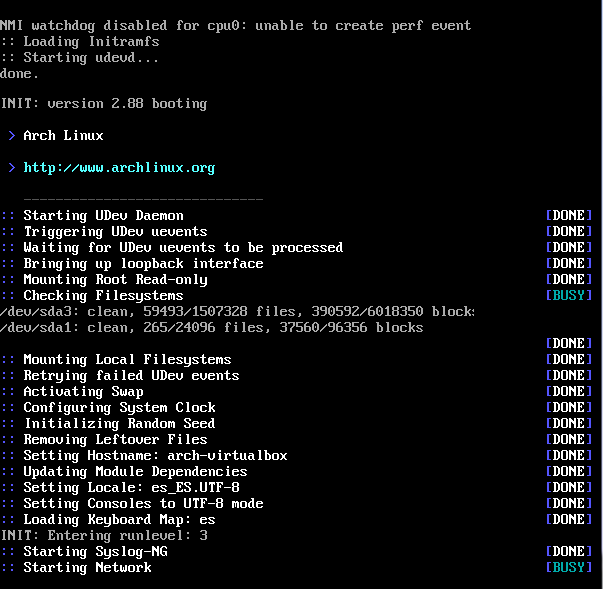
\includegraphics[scale=0.33]{img2/archlinux-boot.png}
\end{frame}


%%%%%%%%%%%%%%%%%%%%%%%%%%%%%%%%%%%%%%%%
%%%%%%%%%%%%%%%%%%%%%%%%%%%%%%%%%%%%%%%%
%%%%%%%%%%%%%%%%%%%%%%%%%%%%%%%%%%%%%%%%
%%%%%%%%%%%%%%%%%%%%%%%%%%%%%%%%%%%%%%%%
%%%%%%%%%%%%%%%%%%%%%%%%%%%%%%%%%%%%%%%%
\begin{frame}
  \frametitle{/sbin/init}

  \begin{itemize}
  \item первый процесс в user space
  \item ответственен за инициализацию системы
  \item реализации: SysVinit, Upstart (Ubuntu), procd (OpenWRT), launchd (Mac OS X)
  \item ...ну и Systemd
  \end{itemize}

\end{frame}


%%%%%%%%%%%%%%%%%%%%%%%%%%%%%%%%%%%%%%%%
%%%%%%%%%%%%%%%%%%%%%%%%%%%%%%%%%%%%%%%%
%%%%%%%%%%%%%%%%%%%%%%%%%%%%%%%%%%%%%%%%
%%%%%%%%%%%%%%%%%%%%%%%%%%%%%%%%%%%%%%%%
%%%%%%%%%%%%%%%%%%%%%%%%%%%%%%%%%%%%%%%%
\begin{frame}[fragile]
  \frametitle{/sbin/init}
  
  \begin{lstlisting}[language=sh]
$ pstree -A
init-+-apache2-+-9*[apache2]
     |         |-apache2---apache2
     |         `-apache2---17*[{apache2}]
     |-cron---cron---sh---php
     |-dbus-daemon
     |-fail2ban-server---8*[{fail2ban-serve}]
     |-6*[getty]
     |-mysqld_safe-+-logger
     |             `-mysqld---20*[{mysqld}]
     |-postfix-policyd
     |-rpc.statd
     |-rsyslogd---3*[{rsyslogd}]
     |-sshd-+-sshd---sshd---bash
     |      `-sshd---sshd---bash---pstree
     `-udevd
  \end{lstlisting}

\end{frame}


%%%%%%%%%%%%%%%%%%%%%%%%%%%%%%%%%%%%%%%%
%%%%%%%%%%%%%%%%%%%%%%%%%%%%%%%%%%%%%%%%
%%%%%%%%%%%%%%%%%%%%%%%%%%%%%%%%%%%%%%%%
%%%%%%%%%%%%%%%%%%%%%%%%%%%%%%%%%%%%%%%%
%%%%%%%%%%%%%%%%%%%%%%%%%%%%%%%%%%%%%%%%
\begin{frame}
  \frametitle{Почему Systemd?}

  \begin{itemize}
  \item Простота использования
  \item Плюшки для разработчиков и мейнтейнеров
  \item Скорость загрузки
  \item Cgroups: изоляция процессов, управление ресурсами
  \item Интеграция подсистем
  \end{itemize}

\end{frame}


%%%%%%%%%%%%%%%%%%%%%%%%%%%%%%%%%%%%%%%%
%%%%%%%%%%%%%%%%%%%%%%%%%%%%%%%%%%%%%%%%
%%%%%%%%%%%%%%%%%%%%%%%%%%%%%%%%%%%%%%%%
%%%%%%%%%%%%%%%%%%%%%%%%%%%%%%%%%%%%%%%%
%%%%%%%%%%%%%%%%%%%%%%%%%%%%%%%%%%%%%%%%
\begin{frame}
  \frametitle{По интерфейсу встречают}

  \begin{columns}
    \begin{column}{.5\textwidth}
      \begin{itemize}
        \item {\tt \# update-rc.d mysql default}
        \item {\tt \# /etc/init.d/mysql start}
        \item {\tt \# /etc/init.d/mysql stop}
        \item {\tt \# /etc/init.d/mysql restart}
        \item {\tt \# update-rc.d -f mysql remove}
      \end{itemize}
    \end{column}

    \begin{column}{.5\textwidth}
      \begin{itemize}
        \item {\tt \# systemctl enable mysql}
        \item {\tt \# systemctl start mysql}
        \item {\tt \# systemctl stop mysql}
        \item {\tt \# systemctl restart mysql}
        \item {\tt \# systemctl disable mysql}
      \end{itemize}
    \end{column}
  \end{columns}

\end{frame}


%%%%%%%%%%%%%%%%%%%%%%%%%%%%%%%%%%%%%%%%
%%%%%%%%%%%%%%%%%%%%%%%%%%%%%%%%%%%%%%%%
%%%%%%%%%%%%%%%%%%%%%%%%%%%%%%%%%%%%%%%%
%%%%%%%%%%%%%%%%%%%%%%%%%%%%%%%%%%%%%%%%
%%%%%%%%%%%%%%%%%%%%%%%%%%%%%%%%%%%%%%%%
\begin{frame}[fragile]
  \frametitle{init скрипт}

  \begin{lstlisting}[language=sh,caption=одна двенадцатая файла /etc/init.d/mysql в Debian 5]
case "${1:-''}" in
  'start')
	sanity_checks;
	# Start daemon
	log_daemon_msg "Starting MySQL database server" "mysqld"
	if mysqld_status check_alive nowarn; then
	   log_progress_msg "already running"
	   log_end_msg 0
	else
	    # Could be removed during boot
	    test -e /var/run/mysqld || install -m 755 -o mysql -g root -d /var/run/mysqld

 	    # Start MySQL! 
  	    /usr/bin/mysqld_safe > /dev/null 2>&1 &

  \end{lstlisting}

\end{frame}


%%%%%%%%%%%%%%%%%%%%%%%%%%%%%%%%%%%%%%%%
%%%%%%%%%%%%%%%%%%%%%%%%%%%%%%%%%%%%%%%%
%%%%%%%%%%%%%%%%%%%%%%%%%%%%%%%%%%%%%%%%
%%%%%%%%%%%%%%%%%%%%%%%%%%%%%%%%%%%%%%%%
%%%%%%%%%%%%%%%%%%%%%%%%%%%%%%%%%%%%%%%%
\begin{frame}[fragile]
  \frametitle{unit файл}

  \begin{lstlisting}[caption=/usr/lib/systemd/system/mysqld.service]
[Unit]
Description=MySQL database server
After=syslog.target

[Service]
User=mysql
Group=mysql

ExecStart=/usr/bin/mysqld --pid-file=/run/mysqld/mysqld.pid 
ExecStartPost=/usr/bin/mysqld-post

Restart=always
PrivateTmp=true

[Install]
WantedBy=multi-user.target
  \end{lstlisting}

\end{frame}


%%%%%%%%%%%%%%%%%%%%%%%%%%%%%%%%%%%%%%%%
%%%%%%%%%%%%%%%%%%%%%%%%%%%%%%%%%%%%%%%%
%%%%%%%%%%%%%%%%%%%%%%%%%%%%%%%%%%%%%%%%
%%%%%%%%%%%%%%%%%%%%%%%%%%%%%%%%%%%%%%%%
%%%%%%%%%%%%%%%%%%%%%%%%%%%%%%%%%%%%%%%%
\begin{frame}
  \frametitle{init-скрипты против unit-файлов}

  \begin{columns}
    \begin{column}{.5\textwidth}
      \begin{itemize}
        \item init-скрипты дают полный контроль над процессом запуска приложения
        \item с точки зрения архитектуры ОС это простое и надежное решение
        \item шаблоны запуска приложений теряются за десятками строк кода
        \item демонизация (скрипты могут запускаться из пользовательских сессий)
        \item реализации пишутся мэйнтейнерами дистрибутивов, а не авторами приложений
        \item дебаг init-скриптов --- вмеру сложно
      \end{itemize}
    \end{column}

    \begin{column}{.5\textwidth}
      \begin{itemize}
        \item Systemd - это еще один слой абстракции
        \item и сам Systemd может непредсказуемо сломаться
        \item простые шаблоны запуска приложений
        \item демонизация в чистом виде становится ненужной
        \item реализации unit-файлов могут поддерживаться авторами приложений
        \item лучшая изоляция процессов за счет использования CGroups
        \item \sout{распараллеливание загрузки системы}
      \end{itemize}
    \end{column}
  \end{columns}

\end{frame}


%%%%%%%%%%%%%%%%%%%%%%%%%%%%%%%%%%%%%%%%
%%%%%%%%%%%%%%%%%%%%%%%%%%%%%%%%%%%%%%%%
%%%%%%%%%%%%%%%%%%%%%%%%%%%%%%%%%%%%%%%%
%%%%%%%%%%%%%%%%%%%%%%%%%%%%%%%%%%%%%%%%
%%%%%%%%%%%%%%%%%%%%%%%%%%%%%%%%%%%%%%%%
\begin{frame}[fragile]
  \frametitle{Cgroups}

  \begin{lstlisting}
/
/system
/system/slim.service
/system/systemd-journald.service
/system/cronie.service
/system/dbus.service
/system/netctl-auto@.service
/system/netctl-auto@.service/netctl-auto@wlan0.service
/system/getty@.service
/system/polkit.service
/system/rtkit-daemon.service
/system/sshd.service
/system/systemd-logind.service
/system/systemd-udevd.service
/user/1000.user/1.session
  \end{lstlisting}

\end{frame}


%%%%%%%%%%%%%%%%%%%%%%%%%%%%%%%%%%%%%%%%
%%%%%%%%%%%%%%%%%%%%%%%%%%%%%%%%%%%%%%%%
%%%%%%%%%%%%%%%%%%%%%%%%%%%%%%%%%%%%%%%%
%%%%%%%%%%%%%%%%%%%%%%%%%%%%%%%%%%%%%%%%
%%%%%%%%%%%%%%%%%%%%%%%%%%%%%%%%%%%%%%%%
\begin{frame}[fragile]
  \frametitle{Cgroups: управление ресурсами}

  \begin{lstlisting}[caption=/usr/lib/systemd/system/example.service]
[Unit]
Description=Example server

[Service]
ExecStart=/usr/bin/example

CPUShares=2048
MemorySoftLimit=1G
#MemoryLimit=1G
BlockIOWeight=500
BlockIOWriteBandwidth=/dev/sda 5M

[Install]
WantedBy=multi-user.target
  \end{lstlisting}

\end{frame}


%%%%%%%%%%%%%%%%%%%%%%%%%%%%%%%%%%%%%%%%
%%%%%%%%%%%%%%%%%%%%%%%%%%%%%%%%%%%%%%%%
%%%%%%%%%%%%%%%%%%%%%%%%%%%%%%%%%%%%%%%%
%%%%%%%%%%%%%%%%%%%%%%%%%%%%%%%%%%%%%%%%
%%%%%%%%%%%%%%%%%%%%%%%%%%%%%%%%%%%%%%%%
\begin{frame}
  \frametitle{Journal}

  \begin{itemize}
  \item journald --- сервис, который занимается сбором, сохранением и отдачей логов;
  \item логи хранятся в бинарном формате
  \item вместе с набором проиндексированных мета-данных (!!!)
  \item и контролем целостности
  \item (но единственная веская причина создания journal'а --- {\tt systemctl status});
  \item работа с логами --- через специальную утилиту {\tt journalctl}\ldots
  \item \ldots или Python-модуль {\tt systemd.journal} (запись и чтение);
  \end{itemize}

\end{frame}


%%%%%%%%%%%%%%%%%%%%%%%%%%%%%%%%%%%%%%%%
%%%%%%%%%%%%%%%%%%%%%%%%%%%%%%%%%%%%%%%%
%%%%%%%%%%%%%%%%%%%%%%%%%%%%%%%%%%%%%%%%
%%%%%%%%%%%%%%%%%%%%%%%%%%%%%%%%%%%%%%%%
%%%%%%%%%%%%%%%%%%%%%%%%%%%%%%%%%%%%%%%%
\begin{frame}[fragile]
  \frametitle{journalctl}
  
  \begin{lstlisting}[language=sh]
# journalctl
Sep 21 12:15:14 jazzcafe systemd[1]: Startup finished in 2.892s
Sep 21 12:15:16 jazzcafe slim[643]: amixer: Unable to find
Sep 21 12:15:17 jazzcafe kernel: wlan0: authenticate with
Sep 21 12:15:17 jazzcafe kernel: wlan0: send auth to 00:22:b0:
Sep 21 12:15:17 jazzcafe kernel: wlan0: authenticated
Sep 21 12:15:17 jazzcafe kernel: iwlwifi 0000:03:00.0 wlan0:
Sep 21 12:15:17 jazzcafe kernel: iwlwifi 0000:03:00.0 wlan0:
Sep 21 12:15:17 jazzcafe kernel: wlan0: associate with 00:22:b0
Sep 21 12:15:17 jazzcafe kernel: wlan0: RX AssocResp from
Sep 21 12:15:17 jazzcafe wpa_actiond[1864]: Interface 'wlan0'
\end{lstlisting}

\end{frame}


%%%%%%%%%%%%%%%%%%%%%%%%%%%%%%%%%%%%%%%%
%%%%%%%%%%%%%%%%%%%%%%%%%%%%%%%%%%%%%%%%
%%%%%%%%%%%%%%%%%%%%%%%%%%%%%%%%%%%%%%%%
%%%%%%%%%%%%%%%%%%%%%%%%%%%%%%%%%%%%%%%%
%%%%%%%%%%%%%%%%%%%%%%%%%%%%%%%%%%%%%%%%
\begin{frame}[fragile]
  \frametitle{journalctl -o verbose}
  
  \begin{lstlisting}[language=sh]
Sat 2013-09-21 12:14:26 FET [s=4e6ebc108450474d9fd3d43b96562483
        _BOOT_ID=0da18fa3d07e43b3af51043d64451f66
        _MACHINE_ID=b4f307d9cadce8040f7d75b30000147a
        _HOSTNAME=jazzcafe
        PRIORITY=5
        SYSLOG_FACILITY=3
        _UID=0
        _GID=0
        _TRANSPORT=syslog
        SYSLOG_IDENTIFIER=wpa_actiond
        SYSLOG_PID=1191
        MESSAGE=Starting wpa_actiond session for interface
        _PID=1191
        _EXE=/usr/bin/wpa_actiond
        _CMDLINE=wpa_actiond -p /run/wpa_supplicant -i wlan0
        _SYSTEMD_CGROUP=/system/netctl-auto@.service/netctl-
        _SYSTEMD_UNIT=netctl-auto@wlan0.service
\end{lstlisting}

\end{frame}


%%%%%%%%%%%%%%%%%%%%%%%%%%%%%%%%%%%%%%%%
%%%%%%%%%%%%%%%%%%%%%%%%%%%%%%%%%%%%%%%%
%%%%%%%%%%%%%%%%%%%%%%%%%%%%%%%%%%%%%%%%
%%%%%%%%%%%%%%%%%%%%%%%%%%%%%%%%%%%%%%%%
%%%%%%%%%%%%%%%%%%%%%%%%%%%%%%%%%%%%%%%%
\begin{frame}[fragile]
  \frametitle{Пишем в журнал}
  
  \begin{lstlisting}
logging.basicConfig(level=logging.DEBUG)

# FROM_SOMEBODY will be sent to journal with every record
hndlr = systemd.journal.JournalHandler(
    level=logging.INFO, FROM_SOMEBODY='WITH_LOVE'
)
logging.root.addHandler(hndlr)

app_user_id = 100500
# oops, APP_USER_ID won't be sent to journal
logging.warning('Session started', extra={'APP_USER_ID': app_user_id})

# APP_USER_ID will be sent to journal
systemd.journal.send('Session ended', APP_USER_ID=str(app_user_id))
  \end{lstlisting}

\end{frame}


%%%%%%%%%%%%%%%%%%%%%%%%%%%%%%%%%%%%%%%%
%%%%%%%%%%%%%%%%%%%%%%%%%%%%%%%%%%%%%%%%
%%%%%%%%%%%%%%%%%%%%%%%%%%%%%%%%%%%%%%%%
%%%%%%%%%%%%%%%%%%%%%%%%%%%%%%%%%%%%%%%%
%%%%%%%%%%%%%%%%%%%%%%%%%%%%%%%%%%%%%%%%
\begin{frame}
  \frametitle{Сокет-активация}

  \begin{itemize}
  \item вместо демона запускается легковесный процесс, слушающий сокет
  \item при поступлении данных запускается демон с преинициализированным сокетом
  \item изначально механизм был придуман для ускорения инициализации системы
  \item сама идея позаимствована из launchd
  \end{itemize}

\end{frame}


%%%%%%%%%%%%%%%%%%%%%%%%%%%%%%%%%%%%%%%%
%%%%%%%%%%%%%%%%%%%%%%%%%%%%%%%%%%%%%%%%
%%%%%%%%%%%%%%%%%%%%%%%%%%%%%%%%%%%%%%%%
%%%%%%%%%%%%%%%%%%%%%%%%%%%%%%%%%%%%%%%%
%%%%%%%%%%%%%%%%%%%%%%%%%%%%%%%%%%%%%%%%
\begin{frame}[fragile]
  \frametitle{Сокет-активация: простой HTTP-сервер}

  \begin{lstlisting}
class HttpServer(tulip.http.ServerHttpProtocol):
    @tulip.coroutine
    def handle_request(self, message, payload):
        response = tulip.http.Response(self.transport, 200)
        response.add_header('Transfer-Encoding', 'chunked')
        response.add_chunking_filter(1025)
        response.add_header('Content-type', 'text/plain')
        response.send_headers()

        with open(__file__, 'rb') as fp:
            chunk = fp.read(8196)
            while chunk:
                response.write(chunk)
                chunk = fp.read(8196)

        response.write_eof()
  \end{lstlisting}

\end{frame}


%%%%%%%%%%%%%%%%%%%%%%%%%%%%%%%%%%%%%%%%
%%%%%%%%%%%%%%%%%%%%%%%%%%%%%%%%%%%%%%%%
%%%%%%%%%%%%%%%%%%%%%%%%%%%%%%%%%%%%%%%%
%%%%%%%%%%%%%%%%%%%%%%%%%%%%%%%%%%%%%%%%
%%%%%%%%%%%%%%%%%%%%%%%%%%%%%%%%%%%%%%%%
\begin{frame}[fragile]
  \frametitle{Сокет-активация: запускаем HTTP-сервер без сокет-активации}

  \begin{lstlisting}
loop = tulip.get_event_loop()
f = loop.start_serving(HttpServer, '127.0.0.1', 8000)

socks = loop.run_until_complete(f)
print('serving on', socks[0].getsockname())
try:
    loop.run_forever()
except KeyboardInterrupt:
    pass
  \end{lstlisting}

\end{frame}


%%%%%%%%%%%%%%%%%%%%%%%%%%%%%%%%%%%%%%%%
%%%%%%%%%%%%%%%%%%%%%%%%%%%%%%%%%%%%%%%%
%%%%%%%%%%%%%%%%%%%%%%%%%%%%%%%%%%%%%%%%
%%%%%%%%%%%%%%%%%%%%%%%%%%%%%%%%%%%%%%%%
%%%%%%%%%%%%%%%%%%%%%%%%%%%%%%%%%%%%%%%%
\begin{frame}[fragile]
  \frametitle{Сокет-активация: запускаем HTTP-сервер с сокет-активацией}

  \begin{lstlisting}
loop = tulip.get_event_loop()

fd = systemd.daemon.listen_fds()[0]
if not systemd.daemon.is_socket_inet(fd):
    raise Exception('Configuration error')

sckt = socket.fromfd(fd, socket.AF_INET, socket.SOCK_STREAM)
sckt.setblocking(0)
f = loop.start_serving(lambda:HttpServer(loop=loop), sock=sckt)

loop.run_until_complete(f)
print('serving on', sckt.getsockname())
try:
    loop.run_forever()
except KeyboardInterrupt:
    pass
  \end{lstlisting}

\end{frame}


%%%%%%%%%%%%%%%%%%%%%%%%%%%%%%%%%%%%%%%%
%%%%%%%%%%%%%%%%%%%%%%%%%%%%%%%%%%%%%%%%
%%%%%%%%%%%%%%%%%%%%%%%%%%%%%%%%%%%%%%%%
%%%%%%%%%%%%%%%%%%%%%%%%%%%%%%%%%%%%%%%%
%%%%%%%%%%%%%%%%%%%%%%%%%%%%%%%%%%%%%%%%
\begin{frame}[fragile]
  \frametitle{Сокет-активация: останавливаем сервер после 10 секунд неактивности}

  \begin{lstlisting}
class HttpServer(tulip.http.ServerHttpProtocol):
    def __init__(self, *args, **kwargs):
        super(HttpServer, self).__init__(*args, **kwargs)
        self.schedule_shutdown(self._loop)

    @classmethod
    def schedule_shutdown(cls, loop):
        future_sysexit = getattr(cls, '_future_sysexit', None)
        if future_sysexit:
            future_sysexit.cancel()
        cls._future_sysexit = loop.call_later(10, sys.exit)

    @tulip.coroutine
    def handle_request(self, message, payload):
        # [...]
        response.write_eof()
        self.schedule_shutdown(self._loop)
  \end{lstlisting}

\end{frame}


%%%%%%%%%%%%%%%%%%%%%%%%%%%%%%%%%%%%%%%%
%%%%%%%%%%%%%%%%%%%%%%%%%%%%%%%%%%%%%%%%
%%%%%%%%%%%%%%%%%%%%%%%%%%%%%%%%%%%%%%%%
%%%%%%%%%%%%%%%%%%%%%%%%%%%%%%%%%%%%%%%%
%%%%%%%%%%%%%%%%%%%%%%%%%%%%%%%%%%%%%%%%
\begin{frame}[fragile]
  \frametitle{Сокет-активация: unit-файлы}

  \begin{lstlisting}[caption=/usr/lib/systemd/system/httpserver.socket]
[Socket]
ListenStream=127.0.0.1:8000
[Install]
WantedBy=sockets.target
  \end{lstlisting}

  \begin{lstlisting}[caption=/usr/lib/systemd/system/httpserver.service]
[Unit]
Description=Example HTTP server
Requires=httpserver.socket
[Service]
ExecStart=/usr/bin/httpserver

[Install]
WantedBy=multi-user.target
Also=httpserver.socket
  \end{lstlisting}

\end{frame}


%%%%%%%%%%%%%%%%%%%%%%%%%%%%%%%%%%%%%%%%
%%%%%%%%%%%%%%%%%%%%%%%%%%%%%%%%%%%%%%%%
%%%%%%%%%%%%%%%%%%%%%%%%%%%%%%%%%%%%%%%%
%%%%%%%%%%%%%%%%%%%%%%%%%%%%%%%%%%%%%%%%
%%%%%%%%%%%%%%%%%%%%%%%%%%%%%%%%%%%%%%%%
\begin{frame}[fragile]
  \frametitle{Таймеры - полноценная замена cron'а}

  \begin{lstlisting}[caption=/etc/systemd/system/timer-daily.timer]
[Unit]
Description=Daily Timer

[Timer]
OnBootSec=10min
OnUnitActiveSec=1d
#OnActiveSec=, OnStartupSec=, OnUnitInactiveSec=, OnCalendar=
Unit=logrotate.service
  \end{lstlisting}

  \begin{lstlisting}[caption=/etc/systemd/system/timer-daily.target.wants/logrotate.service]
[Unit]
Description=Rotate Logs

[Service]
ExecStart=/usr/bin/logrotate /etc/logrotate.conf
  \end{lstlisting}

\end{frame}


%%%%%%%%%%%%%%%%%%%%%%%%%%%%%%%%%%%%%%%%
%%%%%%%%%%%%%%%%%%%%%%%%%%%%%%%%%%%%%%%%
%%%%%%%%%%%%%%%%%%%%%%%%%%%%%%%%%%%%%%%%
%%%%%%%%%%%%%%%%%%%%%%%%%%%%%%%%%%%%%%%%
%%%%%%%%%%%%%%%%%%%%%%%%%%%%%%%%%%%%%%%%
\begin{frame}
  \frametitle{Будущее Systemd}

  \begin{center}
    {\Huge RHEL 7}

    вторая половина 2013
  \end{center}
\end{frame}


%%%%%%%%%%%%%%%%%%%%%%%%%%%%%%%%%%%%%%%%
%%%%%%%%%%%%%%%%%%%%%%%%%%%%%%%%%%%%%%%%
%%%%%%%%%%%%%%%%%%%%%%%%%%%%%%%%%%%%%%%%
%%%%%%%%%%%%%%%%%%%%%%%%%%%%%%%%%%%%%%%%
%%%%%%%%%%%%%%%%%%%%%%%%%%%%%%%%%%%%%%%%
\begin{frame}
  \frametitle{Настоящее Systemd}

  \begin{itemize}
  \item ArchLinux
  \item Fedora
  \item Mageia
  \item openSUSE
  \item Sabayon
  \item ну или можно повозиться с Debian, Gentoo и др.
  \end{itemize}
\end{frame}


%%%%%%%%%%%%%%%%%%%%%%%%%%%%%%%%%%%%%%%%
%%%%%%%%%%%%%%%%%%%%%%%%%%%%%%%%%%%%%%%%
%%%%%%%%%%%%%%%%%%%%%%%%%%%%%%%%%%%%%%%%
%%%%%%%%%%%%%%%%%%%%%%%%%%%%%%%%%%%%%%%%
%%%%%%%%%%%%%%%%%%%%%%%%%%%%%%%%%%%%%%%%
\begin{finalframe}
  \frametitle{СПАСИБО ЗА ВНИМАНИЕ. ВОПРОСЫ?}
    \begin{block}{Стас Рудаков}
    \par \url{mailto:stas@garage22.net}
    \par \url{https://raw.github.com/nott/talks/systemd_webdev.pdf}
    \end{block}

    \begin{block}
      \par \url{http://freedesktop.org/wiki/Software/systemd/}
      \par \url{http://0pointer.de/blog/projects/the-biggest-myths.html}
      \par \url{http://0pointer.de/blog/projects}
      \par \url{lists.freedesktop.org/archives/systemd-devel/2013-June/011388.html}
    \end{block}

\end{finalframe}

\end{document}

